%This work is licensed under the Creative Commons License Attribution 4.0 International (CC-BY 4.0) 
%https://creativecommons.org/licenses/by/4.0/legalcode 
\documentclass[rgb]{standalone}
\usepackage{tkz-euclide}
\usetikzlibrary{matrix}
\definecolor{myorange}{hsb}{0.0833, 1, 0.8}
\definecolor{mygreen}{hsb}{0.3333, 1, 0.8}
\definecolor{myblue}{hsb}{0.5833, 1, 0.8}
\definecolor{mymagenta}{hsb}{0.8333, 1, 0.8}
\begin{document}
	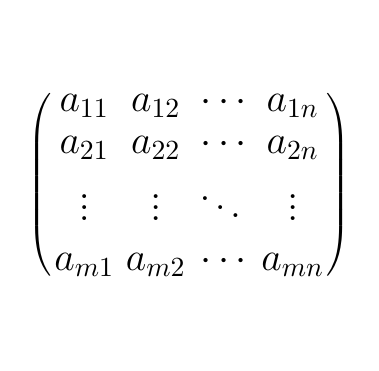
\begin{tikzpicture}[scale=0.5, font=\Large]
		\draw[draw=none] (-4,-4) -- (-4,4) -- (4,4) -- (4,-4) -- cycle;
		\matrix [matrix of math nodes,column sep=-0.25em,outer sep=-7,left delimiter=(,right delimiter=)](){ 
			a_{11} & a_{12} & \cdots & a_{1n}  \\
			a_{21} & a_{22} & \cdots & a_{2n}  \\
			\vdots & \vdots & \ddots\vphantom{a^{1n}} & \vdots \\
			a_{m1} & a_{m2} & \cdots & a_{mn}\vphantom{a^{1n}}    \\
		}; 
	\end{tikzpicture}
\end{document}